\documentclass{article}

\usepackage[final]{nips_2018}

% to avoid loading the natbib package, add option nonatbib:
% \usepackage[nonatbib]{nips_2018}

\usepackage[utf8]{inputenc} % allow utf-8 input
\usepackage[T1]{fontenc}    % use 8-bit T1 fonts
\usepackage{hyperref}       % hyperlinks
\usepackage{url}            % simple URL typesetting
\usepackage{booktabs}       % professional-quality tables
\usepackage{amsfonts}       % blackboard math symbols
\usepackage{nicefrac}       % compact symbols for 1/2, etc.
\usepackage{microtype}      % microtypography

\usepackage{graphicx}
\usepackage{cite}

\title{BLACKE: Body Language Affect Classification by Keypoint Estimation}

\author{Jack (Xiang) Zhou, Gurkaran Aujla, James Bie, Eric Gao, Insoo Rhee\\
	School of Computing Science, 	
	Faculty of Applied Sciences\\
	Simon Fraser University\\
	Burnaby, Canada\\
	\texttt{\{xza194, karana, jbie, emgao, ira3\}@sfu.ca} \\
}

\begin{document}

\maketitle

\begin{abstract}
Current state of the art development in affective classification of people on visual modalities usually focuses on facial expression recognition (FER) but it has some shortcomings in its real world usage. The present approach tackles the affective classification problem in body language by using keypoint estimation as a pre-processing step as opposed to previously used convolutional methods. The approach is found to be plausible with na\"ive neural network classifiers trained over test data. Several implications and pointers to future work are discussed.
\end{abstract}

\section{Introduction}

Affective Computing is a rapidly growing interdisciplinary field that is concerned with interpretations and implications of human emotion in computation. It takes findings and motivations from computing science and psychology into account to piece together approaches to solve problems related to human affect. One of the fundamental problems in Affective Computing is the classification of an individual's emotional state given information about such individual on particular modalities such as text, auditory, behavioural, and visual.

For the visual modality, the present state of the art approach to addressing this problem is by Facial Expression Recognition (FER). The process involves training classifiers that first identifies faces and then taking the images of faces as a means to identify an individual's emotional state through another trained classifier \citep{li2018deep}. The overall method is successful and current approaches with deep neural networks and such can achieve near perfect accuracy ratings on testing data. 

While FER is a successful method, it is not applicable when the face of the individual is not seen, or is covered by objects or body limbs. Observing facial information is often key and a dominant factor when it comes to deciding the current emotional state of a person, and the absence of this information would imply a large increase in variability in evaluating the emotional state of a person. However, in those situations, in order to answer the question of "what is this person feeling", we will have to look at tackling the problem with other available information.

\subsection{Problem Statement}

In the present work, we want to address this shortcoming by identifying the emotional state of an individual in terms of only the body language that they are exhibiting (ie. their posture). Even though the direct link between body language and emotional state is not very apparent, there are still associations linked with understanding the emotional state of a person when observing their body language. 

For example, hands covering face is usually associated with sadness or distress, and extended arms raised high up is usually associated with happiness or surprise. Due to the lack of information posed in this problem, this is inherently a difficult task for humans to perform, in particular with respect to some emotional states over others \citep{schindler2008recognizing} \citep{de2011bodily}. 

Previous work has been done on the topic using a neurologically inspired convolutional classification model that takes in visual data containing both body language and facial expressions (Figure 1) \citep{schindler2008recognizing}.

\begin{figure}[h]
	\centering
	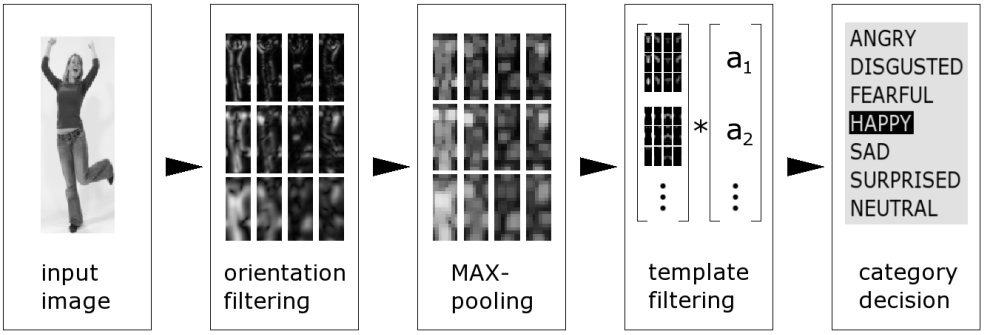
\includegraphics[scale=0.4]{schindlernet}
	\caption{Model used in Schindler et al. 2008}
\end{figure}

The model takes in an input image and applies orientation filtering, pooling, and template filtering on the image before feeding the filtered data into a classifier to arrive at a category decision. It is noteworthy to see that the steps taken to filter and pre-process the image simulates corresponding to various areas of the human visual cortex, going from low level (ex. V1 area) information processing progressively to higher level information processing (ex. V4/IT area).

\subsection{Proposed Work}

While the convolutional filtering approach is plausible and able to perform just as well or better than human test subjects, the model is prone to accounting for extraneous information in its processing steps. The dataset that was used for their experimental work were custom constructed and standardized on neutral backgrounds so the introduction of non-neutral backgrounds (ie. in real life) may be a highly threatening confound.

The present work wishes to approach the same problem by using a different approach to pre-process the input data to a high level representation that primarily accounts for background noise as well as providing other features. Namely, using a representation of the pose of the body in the input image.

The underlying motivation in play here is as follows: Suppose one is visually observing a person, knowing about only the pose that the person is making preserves the relevant information regarding the person's emotional state (Figure 2).

\begin{figure}[h]
	\centering
	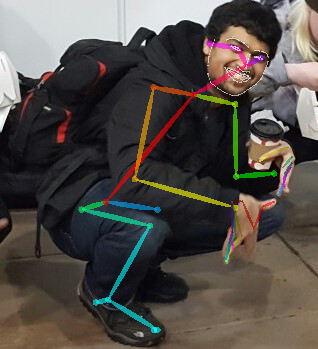
\includegraphics[scale=0.45]{kran}
	\caption{The extracted keypoints of the person's body and face contain the same amount of semantic information regarding the person's emotional state as the full image. Image courtesy of one of our authors Gurkaran Aujla}
\end{figure}

We hypothesize that using a presentation of body posture is a feasible alternative to convolutional pre-processing for classifying emotional states based on just body language. The confirmation of this hypothesis would imply a significant dimensionality reduction to the input data needed for a classifier model, which leads to more compact models and faster training times along with other implications.

\subsection{Keypoint Estimation}

To achieve the goal of representing a pose in a body, we look to applying keypoint estimation with OpenPose \citep{cao2017realtime} \citep{simon2017hand} \citep{wei2016cpm} created by the CMU Perceptual Computing Laboratory, which is open source and freely available for non-commercial use. 

OpenPose is a system that allows for real-time keypoint estimation and detection of human bodies in images and videos. It is capable of finding estimated locations of several body keypoints in the body, hands, and face. It is a capable of doing these simultaneously with multiple people as well. 

Openposes’s	 basic algorithm finds each type of keypoint in all bodies simultaneously, and then finds the connection between these keypoints in a separate neural network. The program can take most image and video formats as inputs, and it will output a variety of formats depending on the configurations. For example, it can output an image with the keypoints overlaid on the people in the image (ex. Figure 2), it can also output JSON files for the keypoints. In the JSON file, it contains the $(x,y)$ coordinates of every bone detected, as well as a confidence rating $c$ for the position of each keypoint expressed as a percentage.

\subsection{Viewpoint Invariance}

As with all work done in computational vision, it is hard to know the exact shape, size and distance of an object in an image as it is only a projection of the original object. The problem of extracting this type of information is called the inverse projection problem, and it is a non-trivial problem.

The ability to account for the inverse projection problem and ultimately achieving viewpoint invariance in models has been a difficult task, especially when the only given information is a two dimensional image most of the time. The state of the art approach in accounting for this problem is by constructing 3D representations of the object seen in the image (for example refer to \citep{shin2018pixels} ). The present work faces many challenges related to this problem and they will be addressed separately in the coming sections.

\section{Approach}

In this section we describe various considerations and challenges toward setting up our models and the overall approach, and the steps taken to account for them.

\subsection{Data Pre-processing}

To prepare any piece of data for the classifiers that we are going to train, the input image has to be fed through OpenPose first to extract a skeleton from the image. One particular advantage to using the Keypoint Estimation approach is that the input dimensions of the image and format do not matter; the output is invariant regardless of these factors. We chose to use the BODY\_25 model which contains 25 body keypoints, as shown in Table 1.

\begin{table}[h]
	\caption{Body Keypoint parts and corresponding enumerations in BODY\_25}
	\centering
	\begin{tabular}{cccccccc}
	\toprule
	0 & 1 & 2 & 3 & 4 & 5 & 6 \\
	Nose & Neck & R\_Shoulder & R\_Elbow & R\_Wrist & L\_Shoulder & L\_Elbow\\	
	\midrule
	8 & 9 & 10 & 11 & 12 & 13 & 14\\
	L\_Wrist & MidHip & R\_Hip & R\_Knee & R\_Ankle & L\_Hip & L\_Knee\\
	\midrule
	15 & 16 & 17 & 18 & 19 & 20 & 21\\
	L\_Ankle & R\_Eye & L\_Eye & R\_Ear & L\_Ear & L\_BigToe & L\_SmallToe\\
	\midrule
	22 & 23 & 24 & 25\\
	L\_Heel &R\_BigToe & R\_SmallToe & R\_Heel\\
	\midrule
	\end{tabular}
\end{table}

Each body keypoint that is extracted from the image comes with a 3-tuple of values $(x,y,c)$ denoting the normalized coordinates (in percentages) of the keypoint and the confidence in the measurement in this point. The total comes to 75 numbers per body, which is significantly less data than an image.

\subsection{Invariance}
Depth perception is a major issue in the present work that has to be addressed. Objects that are closer appear larger than object that are farther away. Humans have a way to account for this issue by preconceived prior knowledge about the world as well as exploiting retinal disparity. However, judging from solely the keypoint information, it is hard to tell whether if someone is tall or if someone is close. The overall translation of the person will also have an impact on what the classifier receives, but the overall position of a person in an image have no bearing on the emotional state of the person.

We propose a transformation over the estimated keypoints that ultimately results in an invariant form that accounts for some of these issues.

\subsubsection{Invariant Form Transformation}

The immediate goal towards a fitting transformation should be that it is translation independent, where any arbitrary set of keypoints should be semantically equivalent to a translated version of those keypoints. The secondary goal is to account for depth perception, which will be done here by discarding information regarding the length of the "bones" (the distance between connected keypoints) in the set of keypoints.

The present approach takes advantage of the fact that the connections between the keypoints in a body exhibit a tree topology (with the nose being the root). That is, each keypoint only has one parent keypoint. Therefore, partial information can be assigned to individual portions and the overall picture can be reconstructed from those pieces of information with a decent level of fidelity. The proposed transformation extracts and only preserves the angle information between keypoints.

We define a mapping from a keypoint tuple $(x_k,y_k,c_k)$ and its parent keypoint tuple $(x_{Pa(k)},y_{Pa(k)},c_{Pa(k)})$ to an invariant polar form $(\theta_k,c'_k)$ as the following:

$$
(\theta_k,c'_k) = \left(\arctan \left(\frac{y_k -y_{Pa(k)}}{x_k -x_{Pa(k)}} \right), \frac{c_k + c_{Pa(k)}}{2}\right)
$$

The resulting image of the transformation forms a new 2-tuple $(\theta, c)$ for all 24 of the non-root keypoints, which contains 48 numbers in total. Although it is not as significant, this transformation poses an even further dimensionality reduction than plainly extracting keypoints.

\subsection{Architecture}

Since we are starting with testing a rudimentary hypothesis, we begin with na\"ive model architectures.

We are working with three different feature sets: estimated keypoints, invariant form and a concatenation of the two. Each of these feature sets will correspond to a neural network that has the same structure except for the input layer. 

The BLACkp network takes the estimated keypoints as inputs, and the BLACangle network takes the invariant form as inputs. Lastly, since it is usually the case that more features leads to better models, we also introduce the BLACkpangle model that takes the concatenation of the inputs to BLACkp and BLACangle as inputs. All three BLAC* networks have two fully-connected hidden layers of size 200 and then 128 neurons, the output is 4 neurons for the four emotional classes that we have in our dataset. All the activation functions being used in the models are Rectified Linear Units (ReLU) with bias terms enabled at every layer. The choice for the sizes of the hidden layers are rather arbitrary but it is slightly motivated from other work being done in FER literature \citep{dachapally2017facial}.

\section{Experiments}

\subsection{Data}

Constructing a dataset was a non-trivial task as it is difficult to find datasets that have faces, full body, and is labelled in a uniform manner. Previous work in this field involved manual construction of data from hired actors \citep{schindler2008recognizing}. For the current work we are piecing together a dataset from various sources. However, since only the posture information will remain, the colorization, image dimensions, and actor identity are not preserved in the keypoint estimation process.

We used the BEAST dataset \citep{de2011bodily} from the Brain and Emotion Laboratory in Maastricht University, which had labelled grayscale images of individuals with their face censored. Images in this dataset are categorized into four emotional categories: Happy, Sad, Angry, and Fearful. We also obtained another dataset from the same laboratory which had the same type of data but colored and larger to include in the dataset that we are piecing together \citep{stienen2012computational}.

Due to the fact that a dominant section of our dataset is standardized and has only four emotional categories, we restricted the amount of classes available in our dataset to be four as well.

From there onwards, the team found suitable images of people online by various means such as image search engines and news articles. The sampled images are then carefully hand-labelled. In order to generate more datapoints, we applied jittering techniques and reflections to transform the data that we already have to achieve a total of 1345 datapoints.

\subsection{Training}

The criterion used is the cross entropy error function, and for every model we apply stochastic gradient descent (SGD) as the optimizer on batch sizes of 5 datapoints each. The learning rate for the SGD algorithm is inversely proportional to the current epoch (ie. $\eta = 1/\mathtt{EPOCH}$) so the decay prevents overstepping minimas in the error surface. For each model, we also try to train with L2-regularization appended to the cross entropy optimizer. In total, we have 6 models that we are training.

The models are trained with the pre-processed data on 1000 epochs for each model, with a 70-30 split between the training data and testing data. The training environment mainly consisted of a Intel Quad-Core i7-6700 with GPU acceleration enabled by a NVIDIA Gefore GTX 1050 Ti.

The resulting test accuracy from training will be compared against each other and against works that have been previously done on the topic (ie. convolutional pre-processing method done in \citep{stienen2012computational} \citep{schindler2008recognizing}).

\subsection{Results}

As we are only concerned about the performance of the models that we are training, only data on test accuracy was collected. The plot of test accuracy progression over training epochs can be seen in Figure 3, and the final results in numbers can be found in Table 2. We found the test accuracy of the BLACkp network subject to L2-Regularization performing the best of all the networks with a test accuracy of 85\%. 

\begin{figure}[h]
\centering
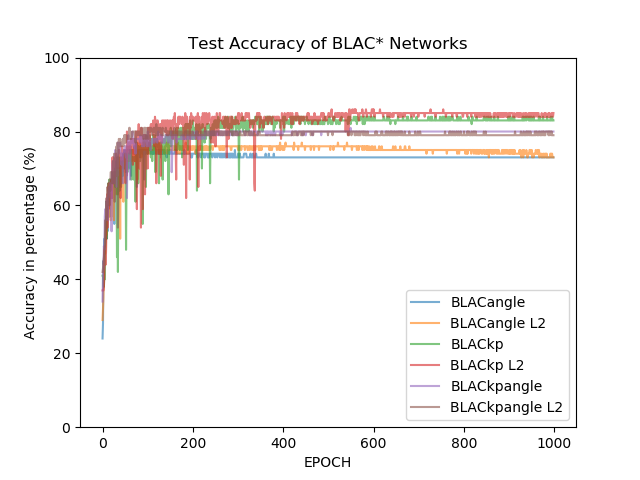
\includegraphics[scale=0.76]{te_acc}
\caption{The test accuracy of all the models trained}
\end{figure}

\begin{table}[h]
	\caption{Test Accuracies of BLAC* Networks}
	\centering
	\begin{tabular}{c|ccc}
	\toprule
	& BLACkp & BLACangle & BLAkpangle \\
	\midrule	
	No Regularization & 84\% & 73\% & 80\%\\
	\midrule
	L2-Regularization & 85\% & 75\% & 79\%\\
	\end{tabular}
\end{table}

\subsubsection{Internal Comparisons}

Regularization did not have a noticeable effect, the only observed differences due to regularization are to the order of at most 2\%. This means that the model is not actively overfitting, passive overfitting may be happening regardless, but we do not know as data was not collected on training accuracy. The size of the dataset is sufficient for our task at hand, and for future work regularization would not be necessary unless the newly proposed architectures are vastly different.

Overall, using estimated keypoints as inputs to a classifier yielded the best results. The combined features network (BLACkpangle) did not perform as well but it did perform better than the network that took our proposed invariant form as inputs.

While regularization did not have a noticeable effect on the model accuracy, we can clearly see that taking in different input features does have an effect on the overall accuracy of the network. This has various implications with respect to the approach that we are taking.

Firstly, this calls for a more informed transformation than the one that we have described in section 2.2.1. The transformation that we have described accounts for some but not all of the issues outlined in section 1.4 and 2.2. Theoretically it should perform better than using solely estimated keypoints because it ought to address some issues that plain keypoints do not.

It is worthy to note that we also tried to train and test all of the BLAC* networks subject to L1-Regularization, but we were met with inexplicable errors leading to overwhelmingly underperforming networks. The test accuracy when networks were subject to L1-regularization dropped significantly after roughly 200 epochs down to baseline performance or lower. For simplicity's sake we decided to not include the related results.

\subsubsection{External Comparisons}

As we are working on a different set of output classes as the ones introduced in \citep{schindler2008recognizing}, we take the marginal test accuracy over all emotional classes of Schindler 2008 as a mode of comparison. The marginal accuracy of the model proposed in Shindler et al. 2008 was 82\%, which was slightly below the testing accuracy of our BLACkp network when subjected to L2-Regularization (85\%).

From this we can confirm our hypothesis and conclude that using keypoint estimation as a means to pre-processing is a feasible alternative to convolutional filtering.

\section{Conclusion}

In the present work we have shown that using keypoint estimation as a preprocessing step is a plausible alternative approach to solving the body language affect classification problem.

\subsection{Future Work}

There are lots more work to be done in this area, especially stemming from the current work. Due to time constraint we were not able to run cross-validation as well as fine-tuning the tradeoff parameter for model regularization. A comprehensive and standardized dataset also needs to be constructed for this problem for future models to be trained effectively. We still firmly believe that an invariant form representation of body language will be able to outperform plain keypoints, so a better and more informed transformation is left as future work.

\section{Contributions}

As with most group projects, each author of this paper contributed a considerable amount of work towards piecing together the project. Jack oversaw the project by organizing and delegating tasks for everyone as well as being the main composer of the paper and poster \footnote{The poster can be found here: \url{https://www.researchgate.net/project/BLACKE}}. After Jack and James formulated the theoretical groundwork in the project, Jack and Insoo went forward with implementing the model and setting up the training environment.

A considerable proportion of the effort went into this project belonged to piecing together a dataset that we can work with. We had the blessing of the Brain and Emotion laboratory in Maastricht University to use their datasets as part of our dataset \citep{de2011bodily}\citep{stienen2012computational}. Aside from the BEAST dataset, Eric and James took the lead in finding images online to include to the dataset and manually hand-labelling them where necessary. After the datset was complete, Gurkaran worked with OpenPose to extract keypoint information from the dataset as well as formulating and implementing the invariant forms for each datapoint. Insoo worked on taking the keypoint data and reorganizing it into a csv file that the models can take in. Eric and Karan worked on a live demo for the presentation.

We would also like to thank Professor Angelica Lim for consultations and guidance toward the design and theoretical groundwork for the project.

\bibliography{references.bib}
\bibliographystyle{plain}

\end{document}